\documentclass[11pt,a4paper]{article}

\usepackage[utf8]{inputenc}
\usepackage[german]{babel}
\usepackage[T1]{fontenc}
\usepackage{amsmath}
\usepackage{amsfonts}
\usepackage{amssymb}
\usepackage{graphicx}
\usepackage{lmodern}
\usepackage{url}
\usepackage{hyperref}

\author{nac}
\title{Chaos macht Schule}
\date{18.12.2017}

\begin{document}

\maketitle

\section{Chaos Computer Club Dresden}
\begin{itemize}
	\item Chaos Computer Club Dresden (=cccdd = c3d2) - \url{https://c3d2.de/space.html}
	\item Projekt: Chaos macht Schule (= CmS) - \url{https://c3d2.de/schule.html}
\end{itemize}

\section{andere Gruppen}
\begin{itemize}
	\item OpenStreetMap - \url{https://wiki.openstreetmap.org/wiki/Stammtisch_Dresden}
	\item Wikipedia - \url{https://de.wikipedia.org/wiki/Wikipedia:Dresden}
	\item Freifunk - \url{https://www.freifunk-dresden.de/}
\end{itemize}

\section{Schulserver Sachsen}
\url{https://www3.sachsen.schule/sbs/startseite/} \\
Bietet verschiedene Kostenfreie Angebote für Schulen, wie: 
\begin{itemize}
	\item Mailinglisten
	\item Wiki 
\end{itemize}

\section{Willkommen in Johannstadt}
\begin{itemize}
	\item Kontaktadresse: \href{mailto:info@willkommen-in-johannstadt.de}{info@willkommen-in-johannstadt.de}
	\item Wir suchen Paten zum Deutsch sprechen und Unterstützung im Alltag für Familien und Einzelpersonen.
	\item Wir suchen Lernpaten für Kinder.
\end{itemize}

\section{Cäsar-Chiffre}
\bigskip
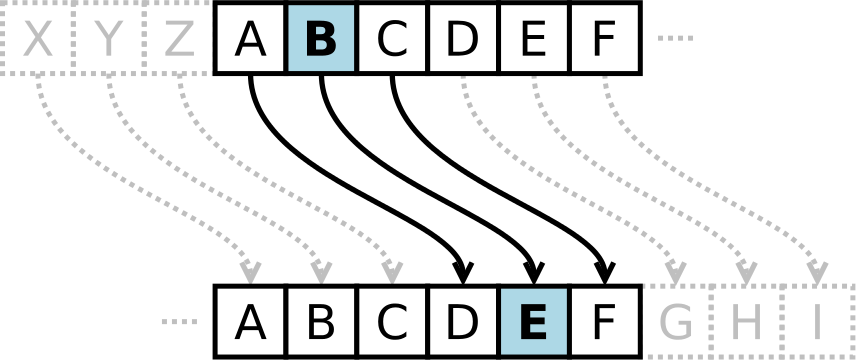
\includegraphics[height=0.1\textheight]{img/caesar.png}

\begin{tabular}{|p{1cm}|p{2cm}|p{3cm}|c|c||}
\hline 
A &  \\ 
\hline 
B &  \\ 
\hline 
C &  \\ 
\hline 
D &  \\ 
\hline 
E &  \\ 
\hline 
F &  \\ 
\hline 
G &  \\ 
\hline 
H &  \\ 
\hline 
I &  \\ 
\hline 
J &  \\ 
\hline 
K &  \\ 
\hline 
L &  \\ 
\hline 
M &  \\ 
\hline 
N &  \\ 
\hline 
O &  \\ 
\hline 
P &  \\ 
\hline 
Q &  \\ 
\hline 
R &  \\ 
\hline 
S &  \\ 
\hline 
T &  \\ 
\hline 
U &  \\ 
\hline 
V &  \\ 
\hline 
W &  \\ 
\hline 
X &  \\ 
\hline 
Y &  \\ 
\hline 
Z &  \\ 
\hline 
\end{tabular} 

\end{document}